% Options for packages loaded elsewhere
\PassOptionsToPackage{unicode}{hyperref}
\PassOptionsToPackage{hyphens}{url}
\PassOptionsToPackage{dvipsnames,svgnames,x11names}{xcolor}
\documentclass[
  11pt,
]{article}
\usepackage{xcolor}
\usepackage[margin=0.85in]{geometry}
\usepackage{amsmath,amssymb}
\setcounter{secnumdepth}{-\maxdimen} % remove section numbering
\usepackage{iftex}
\ifPDFTeX
  \usepackage[T1]{fontenc}
  \usepackage[utf8]{inputenc}
  \usepackage{textcomp} % provide euro and other symbols
\else % if luatex or xetex
  \usepackage{unicode-math} % this also loads fontspec
  \defaultfontfeatures{Scale=MatchLowercase}
  \defaultfontfeatures[\rmfamily]{Ligatures=TeX,Scale=1}
\fi
\usepackage{lmodern}
\ifPDFTeX\else
  % xetex/luatex font selection
\fi
% Use upquote if available, for straight quotes in verbatim environments
\IfFileExists{upquote.sty}{\usepackage{upquote}}{}
\IfFileExists{microtype.sty}{% use microtype if available
  \usepackage[]{microtype}
  \UseMicrotypeSet[protrusion]{basicmath} % disable protrusion for tt fonts
}{}
\makeatletter
\@ifundefined{KOMAClassName}{% if non-KOMA class
  \IfFileExists{parskip.sty}{%
    \usepackage{parskip}
  }{% else
    \setlength{\parindent}{0pt}
    \setlength{\parskip}{6pt plus 2pt minus 1pt}}
}{% if KOMA class
  \KOMAoptions{parskip=half}}
\makeatother
\usepackage{longtable,booktabs,array}
\newcounter{none} % for unnumbered tables
\usepackage{calc} % for calculating minipage widths
% Correct order of tables after \paragraph or \subparagraph
\usepackage{etoolbox}
\makeatletter
\patchcmd\longtable{\par}{\if@noskipsec\mbox{}\fi\par}{}{}
\makeatother
% Allow footnotes in longtable head/foot
\IfFileExists{footnotehyper.sty}{\usepackage{footnotehyper}}{\usepackage{footnote}}
\makesavenoteenv{longtable}
\usepackage{graphicx}
\makeatletter
\newsavebox\pandoc@box
\newcommand*\pandocbounded[1]{% scales image to fit in text height/width
  \sbox\pandoc@box{#1}%
  \Gscale@div\@tempa{\textheight}{\dimexpr\ht\pandoc@box+\dp\pandoc@box\relax}%
  \Gscale@div\@tempb{\linewidth}{\wd\pandoc@box}%
  \ifdim\@tempb\p@<\@tempa\p@\let\@tempa\@tempb\fi% select the smaller of both
  \ifdim\@tempa\p@<\p@\scalebox{\@tempa}{\usebox\pandoc@box}%
  \else\usebox{\pandoc@box}%
  \fi%
}
% Set default figure placement to htbp
\def\fps@figure{htbp}
\makeatother
\setlength{\emergencystretch}{3em} % prevent overfull lines
\providecommand{\tightlist}{%
  \setlength{\itemsep}{0pt}\setlength{\parskip}{0pt}}
\usepackage{amsmath,amssymb}
\usepackage{float}
\usepackage{microtype}
\usepackage{fvextra}
\fvset{breaklines=true}
\usepackage{setspace}
\usepackage{lineno}
\usepackage{etoolbox}
\usepackage{needspace}
\usepackage{xurl}
\AtBeginEnvironment{longtable}{\singlespacing\small}
\AtBeginEnvironment{verbatim}{\singlespacing\small}
\setlength{\emergencystretch}{3em}
\floatplacement{figure}{H}
\DeclareUnicodeCharacter{2212}{\ensuremath{-}}
\DeclareUnicodeCharacter{2264}{\ensuremath{\leq}}
\DeclareUnicodeCharacter{2265}{\ensuremath{\geq}}
\DeclareUnicodeCharacter{2260}{\ensuremath{\ne}}
\DeclareUnicodeCharacter{2208}{\ensuremath{\in}}
\DeclareUnicodeCharacter{221E}{\ensuremath{\infty}}
\DeclareUnicodeCharacter{03B4}{\ensuremath{\delta}}
\DeclareUnicodeCharacter{03BB}{\ensuremath{\lambda}}
\DeclareUnicodeCharacter{03C4}{\ensuremath{\tau}}
\DeclareUnicodeCharacter{03BA}{\ensuremath{\kappa}}
\DeclareUnicodeCharacter{03B3}{\ensuremath{\gamma}}
\DeclareUnicodeCharacter{03B5}{\ensuremath{\varepsilon}}
\DeclareUnicodeCharacter{03C6}{\ensuremath{\phi}}
\DeclareUnicodeCharacter{2124}{\ensuremath{\mathbb Z}}
\DeclareUnicodeCharacter{1D63}{\ensuremath{{}_r}}
\DeclareUnicodeCharacter{2080}{\ensuremath{{}_0}}
\DeclareUnicodeCharacter{208A}{\ensuremath{{}_+}}
\DeclareUnicodeCharacter{208B}{\ensuremath{{}_-}}
\DeclareUnicodeCharacter{207B}{\ensuremath{{}^{-}}}
\DeclareUnicodeCharacter{00B9}{\ensuremath{{}^{1}}}
\DeclareUnicodeCharacter{00B2}{\ensuremath{{}^{2}}}
\DeclareUnicodeCharacter{2074}{\ensuremath{{}^{4}}}
\DeclareUnicodeCharacter{2075}{\ensuremath{{}^{5}}}
\DeclareUnicodeCharacter{2076}{\ensuremath{{}^{6}}}
\DeclareUnicodeCharacter{2192}{\ensuremath{\rightarrow}}
\DeclareUnicodeCharacter{0108}{\ensuremath{\widehat C}}
\DeclareUnicodeCharacter{00C2}{\ensuremath{\widehat A}}

\AtBeginDocument{\doublespacing\linenumbers}
\usepackage{bookmark}
\IfFileExists{xurl.sty}{\usepackage{xurl}}{} % add URL line breaks if available
\urlstyle{same}
% fallback for those not using the hyperref driver hyperxmp:
\makeatletter
\@ifundefined{xmpquote}{\newcommand{\xmpquote}[1]{#1}}{}
\makeatother
\hypersetup{
  colorlinks=true,
  linkcolor={Maroon},
  filecolor={Maroon},
  citecolor={Blue},
  urlcolor={blue},
  pdfcreator={LaTeX via pandoc}}

\author{}
\date{}

\begin{document}

\section{Auditing preprocessing-sensitive allele rankings in predicted
chromatin contact
maps}\label{auditing-preprocessing-sensitive-allele-rankings-in-predicted-chromatin-contact-maps}

Patrick Iben

Independent Researcher, Saint Petersburg, Florida, United States

Corresponding author: Patrick Iben; patrickiben@gmail.com

ORCID: 0009-0005-2443-7973

\subsection{Abstract}\label{abstract}

\textbf{Background:} Preprocessing can change allele rankings derived
from predicted chromatin contact maps without changing the
persistence-interval lifetimes used to summarize each map. We developed
an audit to distinguish this representation effect from evidence of
improved clinical discrimination. We developed mathematical bounds that
use information from uncentered maps to identify which allele will
receive the highest score after centering, while explicitly retaining
unresolved comparisons. A complementary analysis describes how the
distance changes along the centering path.

\textbf{Results:} We evaluated AlphaGenome predictions at 120 discovery
sites and 84 sites in seven new loci, then locked native-only
predictions for a paired IMR-90 test at the same 84 sites. A retained
eleven-gene within-site analysis supplied complementary consequence
controls. In GM12878, centering resolved 138 of 141 native ties and
preserved all 63 strict leaders across discovery and replication. In
IMR-90, strengthened bounds identified 49 of 84 centered leaders versus
seven for simple bounds, adding 42 decisions across six genes with no
contradictions against separately evaluated centered distances; 35 sites
remained unresolved. Numerical endpoint saturation failed in three of
252 comparisons, and both methods abstained at their corresponding
sites. Discovery selected-allele enrichment did not survive multiplicity
correction. Selected-allele credit decreased descriptively after
centering in GM12878 replication and increased in IMR-90;
root-mean-square map baselines exceeded centered topological credit in
both tracks.

\textbf{Conclusions:} The audit identifies when preprocessing makes
topological allele rankings more decisive and which decisions remain
unresolved. Evaluation supports its use on two output tracks of one
prediction model. It does not establish clinical superiority or
experimental structural validity.

\textbf{Keywords:} persistent homology; contact maps; genomic variant
effects; preprocessing; bottleneck distance; numerical validation;
AlphaGenome

\subsection{Background}\label{background}

AlphaGenome predicts molecular outputs from DNA sequence, and
AlphaGenome Atlas exposes variant-effect profiles and an integrated
AlphaGenome Variant Impact score (AVI) {[}1,2{]}. A ranking that places
a clinically selected substitution first can reflect allele effects,
molecular consequence, clinical ascertainment or the representation used
to define the score. Within-site comparisons hold genomic position fixed
while retaining these other sources of separation.

Contact-map topology makes this interpretation problem concrete.
Independently mean-centering reference and alternate maps translates
their persistence diagrams by different amounts. Every interval lifetime
stays unchanged, yet the between-diagram bottleneck distance can change.
Small changes can break tied allele rankings. An analyst already using
these topological summaries therefore needs to distinguish a more
decisive representation from a more informative biological ranking.

We develop an executable audit of this specified preprocessing
operation. Its inputs are persistence diagrams from uncentered maps,
their bottleneck distances and map mean shifts; its outputs include
bounded centered scores, uniquely determined leaders and explicit
unresolved sets. After both endpoint distances are available,
complementary bounds describe how the distance can change throughout the
centering operation. We evaluate the method on spatial discovery data,
prospectively selected new loci and a second output track with
predictions locked before validation. The incorporated eleven-gene Atlas
audit provides the complementary consequence and ascertainment controls.
These form one integrated analysis of the information behind an allele
ranking.

Persistent homology (PH) has established Hi-C applications, including
Sauerwald and colleagues {[}3{]}, topoHiC {[}4{]} and HICTDA {[}5{]},
whose first version awaits peer review. Weighted-network precedents
include Giusti and colleagues {[}6{]} and Petri and colleagues {[}7{]}.
ICE addresses contact-map biases {[}8{]}; shift-invariant and normalized
persistence comparisons address specified transformations {[}9,10,11{]}.
Building on these established methods, we provide an executable audit
that uses uncentered-map information to predict centered allele
rankings, checks those predictions against separately calculated
centered distances, and measures how many comparisons it resolves or
leaves unresolved. Sequence-design work with Akita Semifreddo targets
located boundaries, dots and flames {[}12{]}, highlighting a distinct
future validation target: abstract degree-one intervals are not
automatically located chromatin loops.

\subsection{Methods}\label{methods}

Supporting material covers vertex thinning (Additional file 1), anchor
theory (Additional file 2), Monte Carlo scope (Additional file 3),
paired-track portability (Additional file 4), the retained within-site
audit (Additional file 5), reproducibility details (Additional file 6)
and executable research verification (Additional file 7).

\subsubsection{Predicted maps and
filtration}\label{predicted-maps-and-filtration}

We analyze predicted maps, not observed read counts. AlphaGenome
CONTACT\_MAPS are signed log-fold enrichment over a
genomic-distance-based expectation at 2,048-bp resolution {[}13{]}.
Write this output as \(L\). It is neither a nonnegative count matrix nor
an absolute contact amount. The Atlas contact scorer is a separate
aggregation of local absolute reference--alternate differences {[}14{]};
a vector of track scores is not a genomic-bin matrix. We acquired
spatial maps separately from the retained score caches.

For each fixed set of 512 bins, set the unordered off-diagonal edge
births to \(w_{ij}=-L_{ij}\). This sign convention makes pairs with
greater predicted contact enrichment enter the filtration earlier. At
threshold \(t\), include all vertices and edges with \(w_{ij}\leq t\),
then fill every clique. Full degree-one persistent homology (H1) over
\(\mathbb F_2\) gives \(D_1(w)\). Each interval records the thresholds
at which a one-dimensional topological feature appears and disappears;
\(\mathbb F_2\) specifies arithmetic modulo two. This weighted flag
filtration requires no triangle inequality. On the finite complete
support its degree-one diagram has no essential intervals. Bins,
diagonal exclusion and support are identical within each
reference--alternate comparison. There are 130,816 edges per map.

For two edge arrays on this support, standard filtration stability gives
\(d_B(D_1(w),D_1(v))\leq\lVert w-v\rVert_\infty\) {[}15{]}. Here \(d_B\)
is bottleneck distance, allowing matches to the diagonal; it is not a
distance between Betti curves. A finite filtration cutoff or changed
support requires additional conventions. Read thinning, vertex deletion
and bin aggregation change different objects; none is tested as a
biological endpoint here (Additional file 1). A model enhancing sampled
input, such as DeepHiC {[}16{]}, also inherits uncertainty from that
input.

\subsubsection{Declared anchor path}\label{declared-anchor-path}

For a contact map L, native edge births are \(w=-L\). Here \(a(L)\) is a
single map-specific value, called the anchor, subtracted uniformly from
all entries. Subtracting a scalar \(a(L)\) from every entry of L adds
\(a(L)\) to both coordinates of every full H1 interval. Interval counts
and lifetimes are unchanged. Total persistence, maximum lifetime and the
supremum of the full Betti-one curve are therefore already invariant to
a global additive log-enrichment offset. When L is a known log transform
of positive weights, this offset corresponds to a multiplicative change
in those weights. The interpretation of a scale change depends on the
represented quantity.

Mean centering uses \(a(L)=\operatorname{mean}_{i<j}L_{ij}\) on the
shared off-diagonal support. For reference and alternate native diagrams
\(D_R\) and \(D_A\), define
\(\delta=\operatorname{mean}L_A-\operatorname{mean}L_R\) and

\[f(\lambda)=d_B(D_R,D_A+\lambda\delta),\qquad 0\leq\lambda\leq1.\]

Here addition shifts both birth and death coordinates. Simultaneous
translation of two diagrams leaves their bottleneck distance unchanged,
so \(f(0)\) is the native comparison and \(f(1)\) is the comparison
after independently centering both maps. This path isolates the effect
of that particular preprocessing choice. It does not interpolate
sequences or biological states. The parameter λ is dimensionless; f and
δ have the native log-enrichment coordinate's units.

The construction applies to another scalar anchor by replacing δ with
\(a(L_A)-a(L_R)\). It requires common support and a full filtration.
Clipping, pseudocounts, changes in bin support and finite filtration
windows need separate analysis. Vertex loss is also distinct from a
change in read depth; Additional file 1 gives the finite-bin extinction
argument and its map-specific refinement.

For context, mean centering is a linear operator with exact
supremum-norm constant \(2(1-1/m)\) for m unordered edges. Thus,
centering removes a common offset but can increase the largest
edge-value difference between two maps, by at most this factor.
Normalizing positive weights by their sum likewise selects a diagram
origin after taking logarithms; it leaves full interval lifetimes
unchanged. These identities motivate an audit of the resulting
comparisons.

\pandocbounded{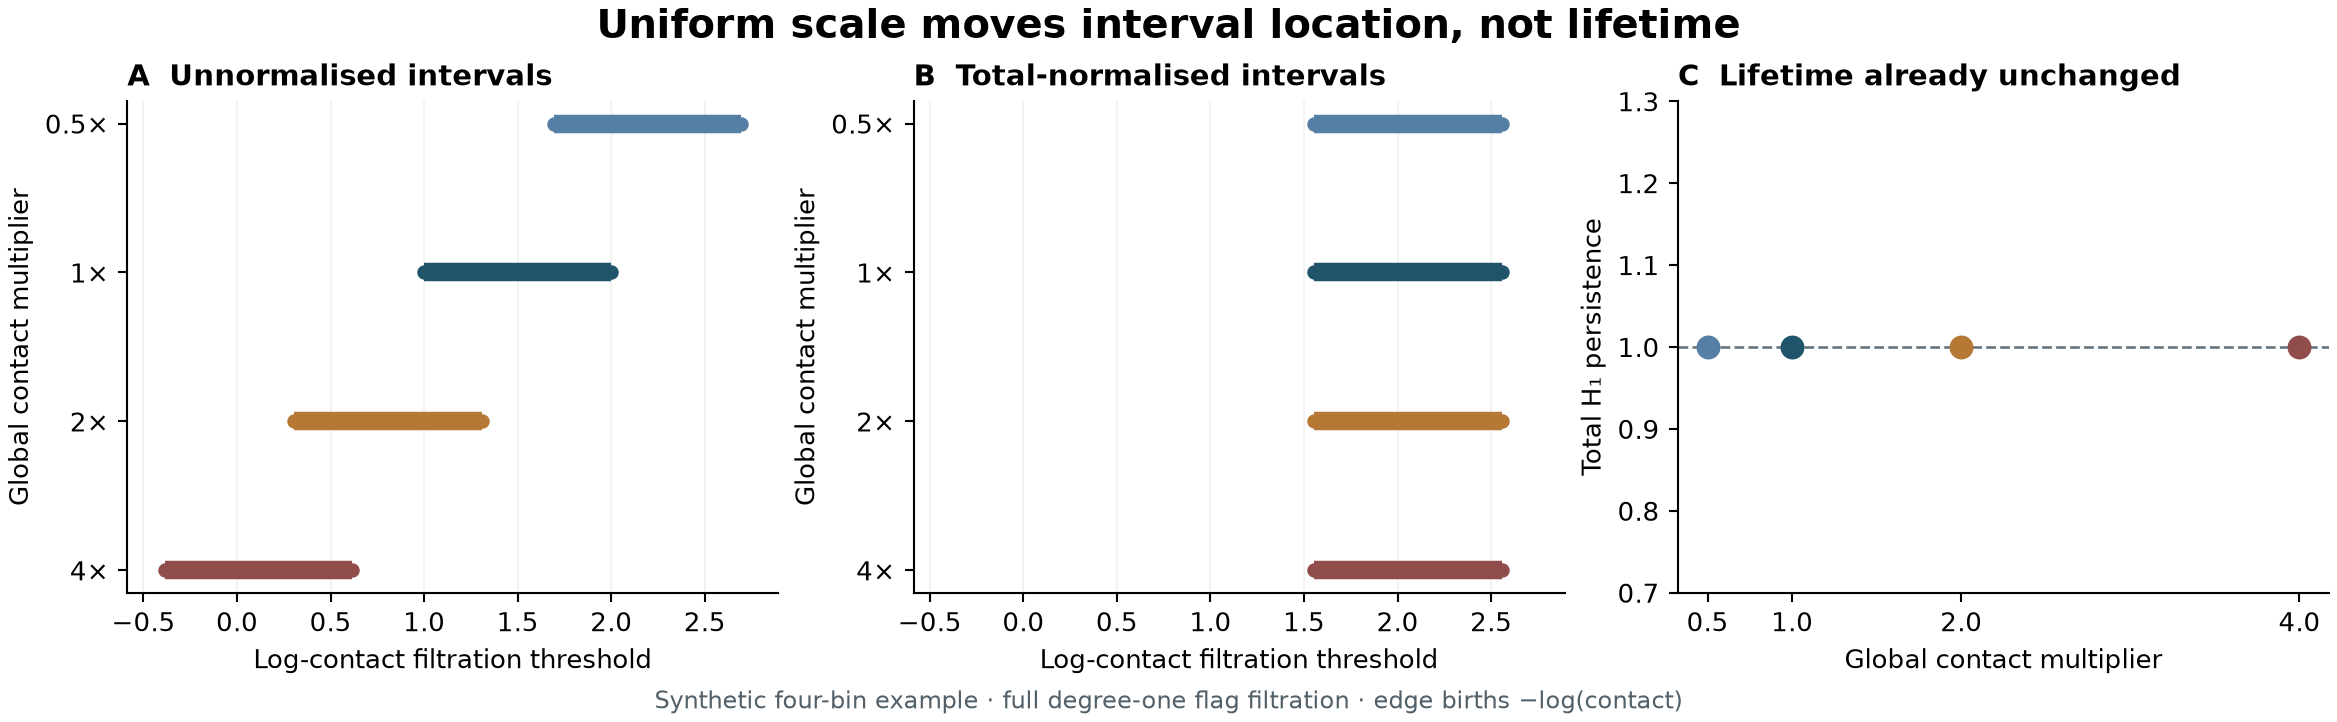
\includegraphics[keepaspectratio,alt={Translation identity illustrated on synthetic data}]{figures/figure_1_scale_and_lifetime.png}}

\par\noindent\begin{minipage}{\linewidth}

\textbf{Figure 1. Translation identity and invariant lifetimes.} A
synthetic four-bin cycle illustrates global scaling before and after
total normalization. Multipliers translate the degree-one interval (A);
normalization aligns it (B); its lifetime is unchanged (C). This
implementation example is not a genomic observation.

\end{minipage}\par

\subsubsection{Endpoint-derived whole-path
envelopes}\label{endpoint-derived-whole-path-envelopes}

These lower and upper bounds use both the uncentered and centered
endpoint distances. They audit the path after endpoint evaluation,
rather than supply the prospective prediction tested below.

\textbf{Proposition (endpoint path bounds).} Write \(T=|\delta|\),
\(A=f(0)\) and \(C=f(1)\). For every λ in {[}0,1{]},

\[\max\{0,A-\lambda T,C-(1-\lambda)T\}
\leq f(\lambda)\leq
\min\{A+\lambda T,C+(1-\lambda)T\}.\]

In particular, \(|C-A|\leq T\). If \(|C-A|=T\), then
\(f(\lambda)=A+\lambda(C-A)\) throughout the segment.

\textbf{Proof.} Matching each interval to its translated copy gives
\(d_B(E+s,E+t)\leq|s-t|\). The triangle inequality makes the distance to
\(D_R\) a 1-Lipschitz function of the shift. Applying this inequality
from each endpoint gives the bounds. When the endpoint difference equals
T, the two bounds coincide. This argument requires neither a fixed
optimal matching nor additional persistence computations.

Exact saturation determines an affine path; near saturation only bounds
its departure. As a function of the diagram shift, finite bottleneck
matching produces a continuous piecewise-affine distance with slopes −1,
0 or +1. With the normalized path parameter \(\lambda\), the
corresponding slopes are \(-T\), 0 or \(+T\). A shift segment contained
entirely within a nonflat piece therefore saturates the endpoint bound.
Additional file 2 gives deficit bounds, matching arguments and
counterexamples. In numerical use, valid endpoint-error enclosures must
widen the envelopes; a small floating-point residual alone is not such
an enclosure.

\subsubsection{Native-only prediction of centered
leaders}\label{native-only-prediction-of-centered-leaders}

The prospective endpoint calculation does \textbf{not} use the centered
distance \(C\). For alternate \(a\), the native inputs are \(D_R,D_a\),
\(A_a=d_B(D_R,D_a)\) and \(T_a=|\delta_a|\). Form the pair of diagrams
\((D_R,D_a+\delta_a)\). Using the maximum-coordinate (\(\ell_\infty\))
distance, compute for each point in either diagram the smaller of its
distance to the nearest point in the other diagram and its own distance
to the diagonal. Let \(H_a\) be the largest of these values. Then
\(H_a\leq d_B(D_R,D_a+\delta_a)\): any complete matching must satisfy
every point's nearest-neighbor requirement. This lower bound does not
enforce a complete matching and cannot replace bottleneck distance.

The audit computes the following intervals before centered matching:

\[
I_a^{\rm simple}=[\max(0,A_a-T_a),\ A_a+T_a],\qquad
I_a^{\rm strong}=[\max(0,A_a-T_a,H_a),\ A_a+T_a].
\]

Here, higher rank means larger centered bottleneck distance. Given
intervals \([L_a,U_a]\) and tie tolerance \(\tau\), return a unique
leader \(i\) only if \(L_i>\max_{j\ne i}U_j+\tau\). Otherwise return an
unresolved set. An outer set of possible top members is
\(\{i:U_i\geq\max_{j\ne i}L_j-\tau\}\); an inner set of necessary top
members is \(\{i:L_i\geq\max_{j\ne i}U_j-\tau\}\). The outer set need
not be sharp because score dependencies are ignored. All interval and
set statements are conditional on valid bounds.

\textbf{Algorithm 1: native-only centered-ranking audit.} (1) Compute
native diagrams, native distances and mean shifts on common support. (2)
Construct the simple intervals. (3) Query nearest neighbors in the
shifted diagrams to construct \(H_a\) and intersect the lower bounds.
(4) Apply the tolerance-aware leader and set rules, retaining every
unresolved site. (5) Save the complete predictions. (6) For evaluation,
compute centered bottleneck distances separately and check score
coverage, top-set inclusion and leader agreement. Steps 1--5 require no
centered matching and no clinical labels; step 6 is the validation
target.

The empirical increment is the number of additional unique leaders
resolved by step 3. Because the strengthened lower bound cannot
decrease, retaining simple-bound decisions is structural, rather than
independent evidence of performance. These are centered-endpoint
decisions. A stricter native-margin condition, \(A_i-A_j>T_i+T_j+\tau\)
for every competitor, can guarantee the same leader throughout the path.
The witness endpoint test does not by itself supply that whole-path
guarantee. No net runtime speedup is inferred from avoiding centered
matching in the prediction stage.

An increasing-branch witness satisfying \(H_a=A_a+T_a\) meets the upper
bound. A decreasing branch needs a different upper witness; we abstain
when the available bounds are insufficient. Neither the scalar native
distance nor the mean shift determines the direction: for
\(D=\{(0,4)\}\) and \(E_\pm=\{(\pm1,4\pm1)\}\), both native distances
are one, but the same shift \(1/4\) yields \(5/4\) and \(3/4\).
Multiplicity also matters: two copies of \((0,4)\) versus one give
nearest-neighbor lower bound zero and bottleneck distance two.
Additional file 2 develops these limitations.

The implemented intervals subtract \(10^{-12}\) from lower bounds and
add it to upper bounds. This is a practical allowance on stored
floating-point diagrams, not a complete real-arithmetic enclosure. The
theoretical guarantees and observed agreement must be read with that
distinction. We use ``identified leader'' for a numerical prediction
validated against the separately computed endpoint, not a clinically
correct allele.

\subsubsection{Evaluation design and separation of prediction from
validation}\label{evaluation-design-and-separation-of-prediction-from-validation}

\textbf{Table 1. Evaluation stages and timing.} The paired track test
reuses sites; it is not a third independent cohort.

{\def\LTcaptype{none} % do not increment counter
\begin{longtable}[]{@{}
  >{\raggedright\arraybackslash}p{(\linewidth - 4\tabcolsep) * \real{0.2000}}
  >{\raggedright\arraybackslash}p{(\linewidth - 4\tabcolsep) * \real{0.3700}}
  >{\raggedright\arraybackslash}p{(\linewidth - 4\tabcolsep) * \real{0.4300}}@{}}
\toprule\noalign{}
\begin{minipage}[b]{\linewidth}\raggedright
Stage
\end{minipage} & \begin{minipage}[b]{\linewidth}\raggedright
Input and scope
\end{minipage} & \begin{minipage}[b]{\linewidth}\raggedright
Timing and target
\end{minipage} \\
\midrule\noalign{}
\endhead
\bottomrule\noalign{}
\endlastfoot
Retained within-site audit & Atlas score profiles in 11 genes; initial
120 sites, 384 pool-replication and 1,713 expanded-panel primary
positions & Original analysis families; expanded-panel plan public
before score retrieval \\
Spatial discovery & GM12878; 120 sites in 4 loci; 360 alternate
comparisons & Local declaration before spatial analysis; primary
centered selected-allele credit; path/witness analysis afterward \\
New-locus spatial replication & GM12878; 84 sites in 7 new loci; 252
comparisons & Cohort/protocol hashed before maps; saturation and ranking
diagnostics; witness increment compared afterward \\
Paired track portability & IMR-90 at the same 84 replication sites; 252
comparisons & Protocol before acquisition; bounds, predicted leaders and
unresolved sets locked before centered-distance evaluation; primary
additional leader coverage \\
\end{longtable}
}

Discovery used ClinVar-selected pathogenic or likely pathogenic coding
substitutions in \emph{DNM1} (20), \emph{PCCA} (15), \emph{PCCB} (27)
and \emph{MMUT} (58) {[}17{]}. Each coordinate has three non-reference
substitutions. The replication selected 12 sites each in \emph{ASS1},
\emph{BAP1}, \emph{BRCA2}, \emph{HFE}, \emph{RB1}, \emph{SCN5A} and
\emph{TSC1} by deterministic hashing within consequence strata, with
proportional residual allocation after reserving one site per nonempty
stratum. All reference bases were checked against GRCh38. This
gene-balanced design oversamples rare consequences. Windows did not
overlap discovery windows or another selected gene, but overlapped
substantially within genes: there are seven new locus regions, not 84
independent regions. The loci had historical nonspatial scorer results;
prospective status concerns the specified new spatial outcomes.

GM12878 in situ Hi-C (4dn:4DNFIXP4QG5B; EFO:0002784) was selected before
inspecting spatial allele results. AlphaGenome ALL\_FOLDS returned 512 ×
512 maps over 1,048,576-bp variant-centered windows. IMR-90
(4dn:4DNFIJTOIGOI; EFO:0001196) was selected from metadata as a distinct
cell context with the same assay and resolution. Both tracks were
requested together in all 252 portability calls. Thus this is a paired
second-track test within one model, not an independent architecture,
new-locus holdout or experimental assay.

For IMR-90, all 84 sites' native diagrams, distances, mean shifts,
bounds and predictions were saved and hashed before any centered
bottleneck evaluation. Technical transfer required complete acquisition,
no validation failures and positive additional coverage. The fixed
operational benchmark required at least 17 additional leaders across at
least four genes, no contradicted decisions and no lost simple
decisions. Seventeen was selected as half the earlier 34-site GM12878
gain; it is a utility threshold, not a powered statistical or clinical
criterion. Primary tie tolerance was \(10^{-6}\), with 0 and \(10^{-5}\)
sensitivities. The benchmark was not revised after results.

The tie tolerance governs ranking decisions; the saturation tolerance is
a separate diagnostic of the endpoint bound. Numerical endpoint
saturation used \(\bigl||C-A|-|\delta|\bigr|\leq10^{-10}\), with tiny
shifts reported separately. Direct midpoint calculations were fixed for
all three alternates at the smallest-hash selected site in each
replication gene: 21 checks per track. After IMR-90 results, a separate
diagnostic protocol specified seven direct distances at
\(\lambda=0,0.1,0.25,0.5,0.75,0.9,1\) for all three nonsaturating
comparisons. Those outcome-selected checks are exploratory and did not
alter the locked primary analysis (Additional file 4).

\subsubsection{Clinical-label summaries and baseline
comparisons}\label{clinical-label-summaries-and-baseline-comparisons}

For the 120-site spatial discovery analysis, the protocol was recorded
before analysis of the new spatial outcomes, with knowledge of the
earlier profile audit. It is a local exploratory declaration, not a
public preregistration. Its primary endpoint was selected-allele
fractional top credit under mean-centered H1 distance. At each site, the
selected allele received credit \(1/k\) if it was among \(k\) alternates
whose scores were within an absolute tolerance of \(10^{-6}\) of the
maximum, and zero otherwise. Thus, an outright top rank earned 1, a
two-way top tie earned 1/2, and a three-way tie earned 1/3. The rank
filtration groups equal edge values and replaces each birth by the
fraction of edges with strictly smaller native birth, retaining stronger
contacts first (Additional file 2). Native enrichment, rank enrichment
and the two-sided centered-minus-native paired credit contrast completed
a four-test family. Exact ties and tolerance 10⁻⁵ were declared
descriptive sensitivities.

Under the primary null, each site's selected label is drawn
independently and uniformly from its three alternatives, conditional on
all maps. Expected fractional credit is 1/3 even with ties. The paired
null uses the same label for both representations and tests absolute
deviation around its conditional expectation. Dynamic-programming
convolution on the sixth-credit lattice evaluates the finite null
distribution. An initial float64 implementation agreed with independent
exhaustive-enumeration checks within 3.22 × 10⁻¹⁵. A separate
implementation then reconstructed all sixteen tests with integer
polynomial coefficients and exact rational probabilities, including
paired expectations, inclusive tails and multiplicity adjustments; its
largest discrepancy from the reported floating values was 6.83 × 10⁻¹⁶.
This certifies the label-probability arithmetic conditional on the
computed credits, not the map predictions or the scientific null. Holm
{[}18{]} and Benjamini--Yekutieli (BY) {[}19{]} adjustments cover all
four main tests. The product-label model does not establish biological
independence among overlapping windows or sites in the same gene.

Three sensitivity nulls were fixed: consequence matching;
transition/transversion weights 4/1 with an additional factor of ten for
CpG transitions; and both together. Consequence matching retains all 120
sites, including 26 with a unique eligible label and thus deterministic
contributions. Applying the four tests under the primary null and each
of the three sensitivity nulls gives sixteen tests, all reported with an
additional Holm adjustment. These weights are assumptions, not measured
clinical ascertainment probabilities. Coordinate-sensitive map
differences and a consequence-severity rule are descriptive baselines.
The prior 66-comparison profile family remains separate.

For every representation we compare fractional selected-allele credit,
not validated pathogenic-versus-benign accuracy. An unselected
alternative is not necessarily benign. Absolute mean change, native and
centered root-mean-square (RMS) map differences, maximum edge change,
interval count and lifetime differences, and native distance plus/minus
absolute mean shift provide descriptive baselines. No new
clinical-enrichment testing family was introduced for spatial
replication or portability. Gene-level and leave-one-gene-out summaries
describe concentration, without treating overlapping windows as
independent biological samples.

The retained Atlas audit evaluated 22 scorers in three geometries with
within-site randomization, declared multiplicity families and
consequence/mutation sensitivities. AVI includes AlphaMissense and
consequence-related features {[}2,20,21{]}. Its reported 9,999-draw
tests use plus-one p-values {[}22{]}, Benjamini--Hochberg (BH) {[}23{]}
and specified BY {[}19{]} corrections; several highlighted cells reach
the Monte Carlo floor. Additional files 3 and 5 preserve the complete
methods, ascertainment, baselines and adverse results. The publicly
deposited expanded-panel plan preceded score retrieval {[}24{]}; the
original reproducibility package is archived {[}25{]}.

\subsubsection{Computation, verification and AI
assistance}\label{computation-verification-and-ai-assistance}

Ripser computed full H1 without interval censoring. GUDHI 3.13.0 CGAL
(\(e=0\)) and Hera (approximation parameter zero) supplied bottleneck
matching, with per-record solver provenance and cross-solver checks.
``Exact matching'' refers to the supplied diagram coordinates, not model
accuracy or elimination of floating-point error. Added float32
filtration-conversion errors were recorded separately. AlphaGenome
client 0.9.0 used the ALL\_FOLDS alias; an immutable server weight
revision and model-training independence were not established.

Stored-map re-execution in a fresh environment covered all 204 GM12878
spatial sites. The sixteen conditional label tests were independently
recomputed, and the retained historical analyses were rerun. For IMR-90,
an unmodified reference-engine replay covered all 84 sites; separate
brute-force nearest-neighbor code checked every witness and
independently reconstructed rankings and rational credits. The replay
uses the same persistent-homology implementation, so it does not test
agreement between different algorithms for constructing the diagrams.
Known-answer controls include increasing, turning, flat, zero-shift and
multiplicity cases. Additional file 6 records execution, solver and
preservation details. The public MIT-licensed Anchor Audit Toolkit
implements the bound calculations and a browser demonstration
{[}26,27{]}; the research-data access status is stated separately below.

Generative artificial intelligence (AI) through OpenAI Codex assisted
study and audit-procedure development; mathematical derivation and
adversarial checking; code for acquisition, processing, statistics and
verification; manuscript drafting and revision; and literature/source
checks. Qwen3.8 assisted earlier manuscript drafting. Author-supplied
quality-control reports were generated with Qwen3.8-Max; accepted
suggestions were checked against the source files and underlying
artifacts before revision. These checks supplement author review rather
than constitute external peer review. AlphaGenome generated the
molecular predictions analyzed here, which are model outputs rather than
experimental measurements. The author is responsible for the submitted
work; no AI system is an author.

\subsection{Results}\label{results}

\subsubsection{Prospective centered-leader
coverage}\label{prospective-centered-leader-coverage}

\textbf{Table 2. Centered-leader coverage at tie tolerance \(10^{-6}\).}
All reported leaders agreed with independently evaluated centered
matching. GM12878 increments were compared after those outcomes; IMR-90
predictions were locked first.

{\def\LTcaptype{none} % do not increment counter
\begin{longtable}[]{@{}
  >{\raggedright\arraybackslash}p{(\linewidth - 6\tabcolsep) * \real{0.3700}}
  >{\raggedleft\arraybackslash}p{(\linewidth - 6\tabcolsep) * \real{0.2100}}
  >{\raggedleft\arraybackslash}p{(\linewidth - 6\tabcolsep) * \real{0.2100}}
  >{\raggedleft\arraybackslash}p{(\linewidth - 6\tabcolsep) * \real{0.2100}}@{}}
\toprule\noalign{}
\begin{minipage}[b]{\linewidth}\raggedright
Quantity
\end{minipage} & \begin{minipage}[b]{\linewidth}\raggedleft
GM12878 discovery
\end{minipage} & \begin{minipage}[b]{\linewidth}\raggedleft
GM12878 replication
\end{minipage} & \begin{minipage}[b]{\linewidth}\raggedleft
IMR-90 paired test
\end{minipage} \\
\midrule\noalign{}
\endhead
\bottomrule\noalign{}
\endlastfoot
Sites & 120 & 84 & 84 (same replication sites) \\
Simple-bound leaders & 45 & 18 & 7 \\
Strengthened-bound leaders & 89 & 52 & 49 \\
Additional leaders & 44 & 34 & 42 \\
Unresolved after strengthening & 31 & 32 & 35 \\
Contradicted leaders & 0 & 0 & 0 \\
\end{longtable}
}

The prospective IMR-90 calculation increased decision coverage from 7/84
to 49/84, adding 42 leaders (50 percentage points) across six genes.
There were no score-interval failures, ranking-set failures or
contradicted leader predictions. Thirty-five sites remained unresolved.
Unresolved denotes insufficient separation of the bounds; it does not
necessarily indicate a tie in the directly computed centered scores.
Gains were ASS1 7, BAP1 11, BRCA2 7, HFE 4, RB1 0, SCN5A 6 and TSC1 7.
Removing any one gene retained 31--42 additional decisions. The frozen
technical and operational criteria were met. The increment was 43 at
zero tolerance and 35 at \(10^{-5}\), again without validation failures.
These are observed agreements on stored diagrams, not estimates of
clinical accuracy or a population error bound.

All 252 paired calls succeeded on the first attempt. All repeated
references were identical; every contemporary GM12878 reference and
alternate array matched its historical counterpart exactly, whereas
every paired IMR-90 map differed from GM12878. Delivered values in both
tracks were bfloat16-representable. Equality at the queried inputs
supports the contemporaneous comparison but does not identify immutable
weights. Independent brute-force witness calculation agreed exactly in
all 252 comparisons. Reference-engine replay matched all 3,696 recorded
field and array comparisons exactly, including 336 full persistence
diagrams (Additional files 4 and 6).

\pandocbounded{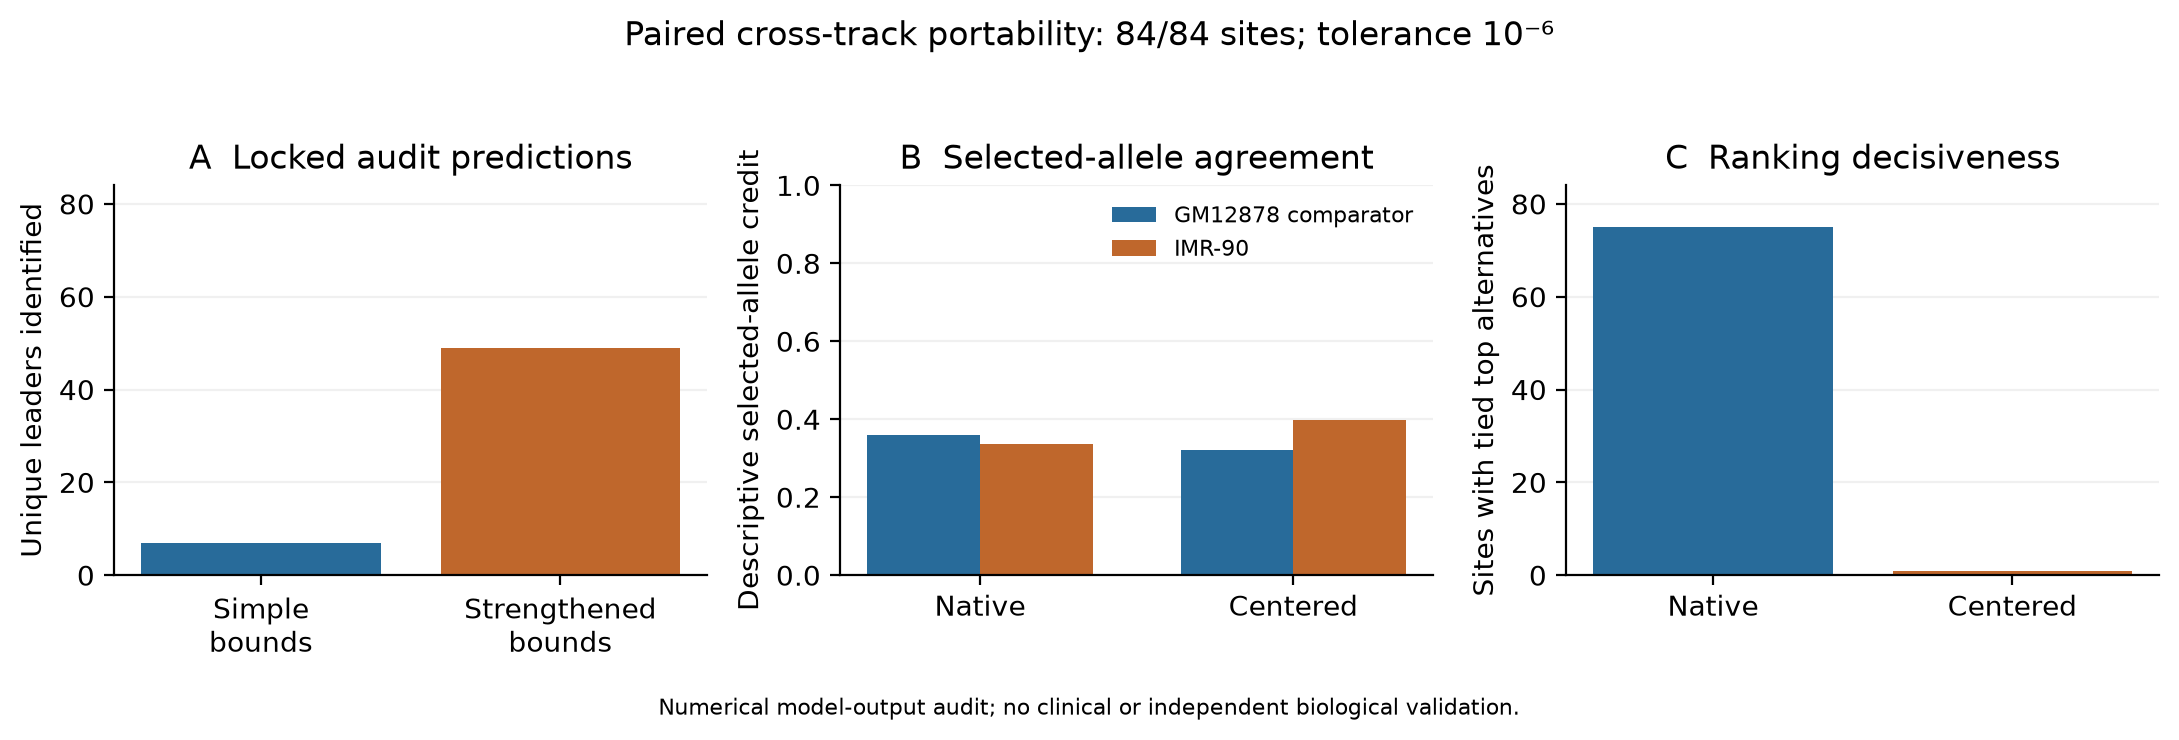
\includegraphics[keepaspectratio,alt={Paired cross-track decision coverage and descriptive rankings}]{figures/figure_2_track_portability.png}}

\par\noindent\begin{minipage}{\linewidth}

\textbf{Figure 2. Paired cross-track decision coverage and descriptive
rankings.} A: unique leaders identified by locked simple and
strengthened bounds before centered evaluation. B: descriptive
native/centered selected-allele credit in the two tracks. C: IMR-90
native and centered tied top sets. Endpoints are computed directly. The
tracks share sites and model architecture; no clinical-accuracy interval
or runtime advantage is implied.

\end{minipage}\par

\subsubsection{Saturation, exceptions and tie
resolution}\label{saturation-exceptions-and-tie-resolution}

Across GM12878 discovery and replication, all 612 comparisons
numerically saturated the endpoint translation bound, with maximum
residuals \(2.08\times10^{-16}\) and \(2.22\times10^{-16}\). Centering
increased 278/360 discovery distances and 182/252 replication distances,
decreasing the remainder. The 21 fixed replication midpoint checks
differed from the straight lines joining the endpoint distances (the
endpoint chords) by at most \(8.33\times10^{-17}\). These finite checks
support the numerical affine description on the computed diagrams. They
do not prove exact equality for unexposed model outputs.

Universal saturation did not transfer to IMR-90: 249/252 comparisons
passed, with no tiny shifts. All three exceptions occurred in RB1; the
maximum deficit was 0.002583775382. Both simple and strengthened bounds
had already abstained at all three corresponding sites. Thus the
witness's distinct contribution is its additional coverage elsewhere,
not unique detection of these exceptional paths.

All 21 prespecified IMR-90 midpoint checks passed both chord and
envelope tolerances; one sampled the effectively flat exception. A
nonsaturating path can still be straight: when a nonzero shift leaves
the distance constant, the endpoint change is zero rather than the full
shift magnitude. Subsequent direct evaluations at seven fixed lambda
values showed two paths changing direction on the sampled grid, with
maximum chord departures 0.000903377 and 0.001291888; the third was flat
within \(10^{-12}\). All 21 exploratory values remained inside the
endpoint envelopes. This diagnoses the sampled behavior without
identifying exact turning locations, matching identities or unmeasured
intermediate rankings (Additional file 4).

At tolerance \(10^{-6}\), centering resolved 72 of 75 discovery ties and
all 66 GM12878 replication ties, preserving all 45 and 18 strict native
leaders. Every centered top set remained inside its native top set; no
strict leader reversed. The simple margin bound supported those leaders
throughout the path. In IMR-90, centering resolved 74 of 75 native ties
and preserved all nine strict leaders. Interval lifetimes remained
unchanged in every map by the translation identity. The repeated
increase in unique rankings is therefore a representation effect whose
clinical interpretation needs separate evidence.

\pandocbounded{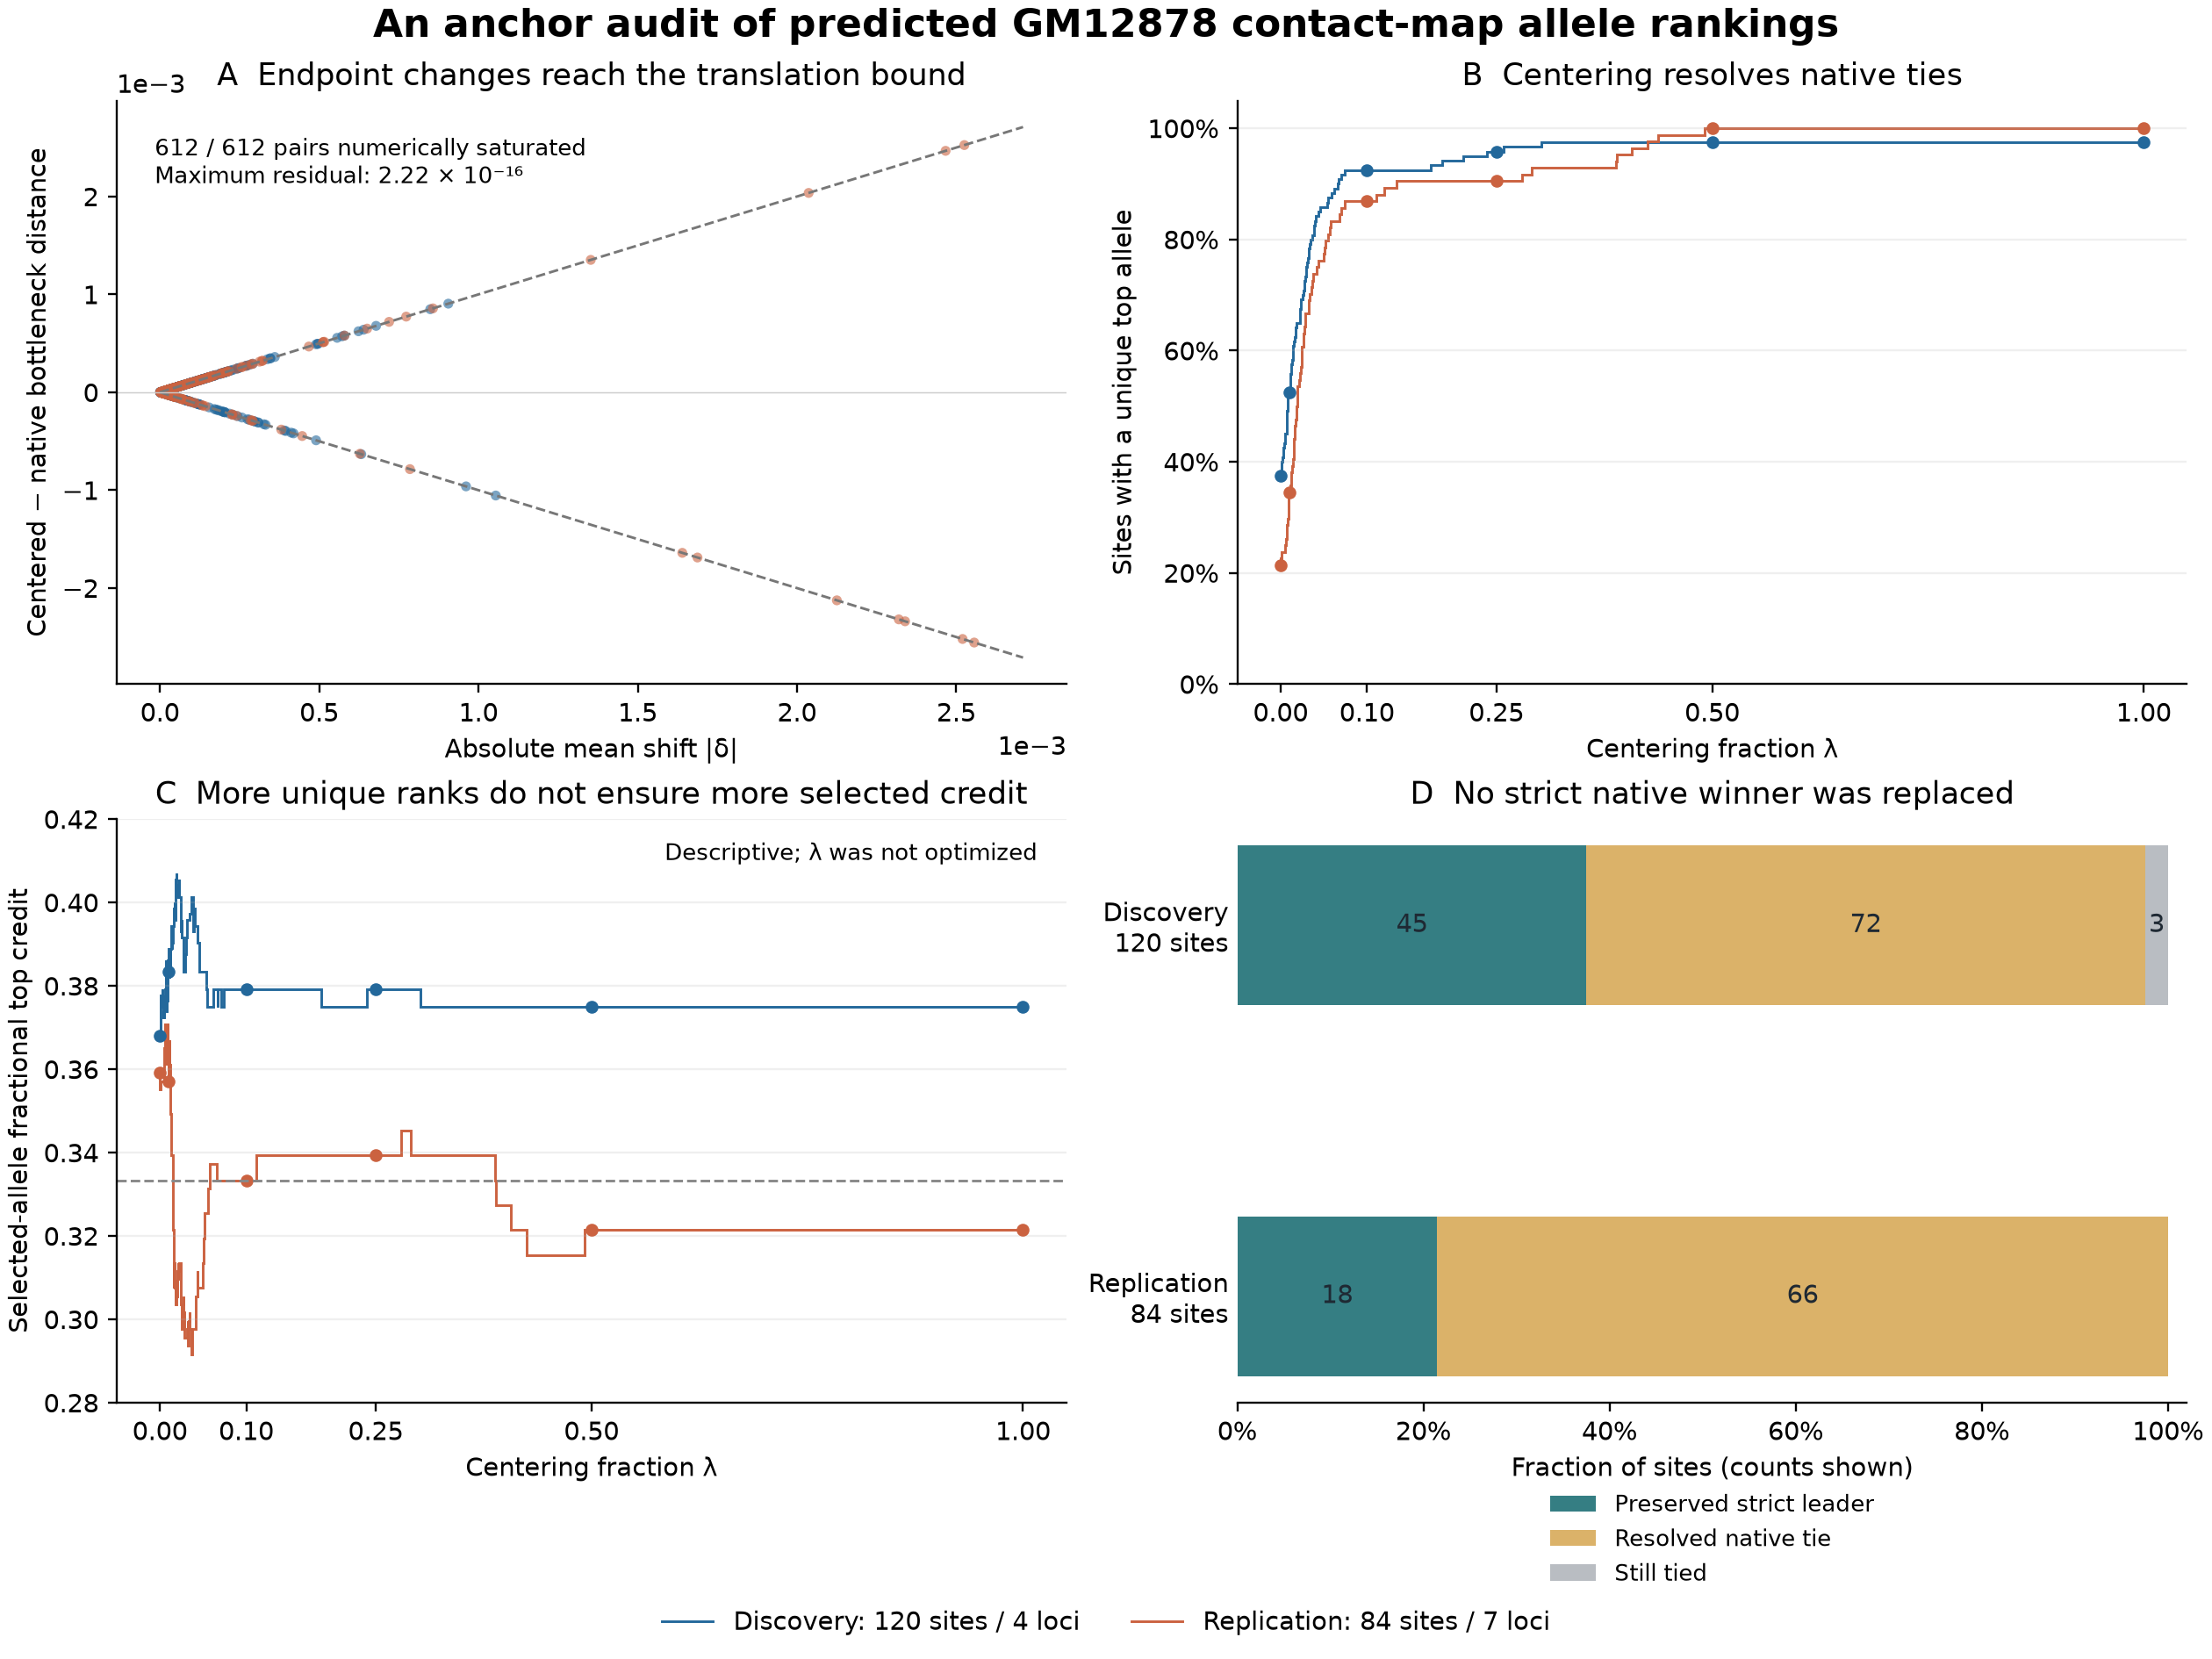
\includegraphics[keepaspectratio,alt={Anchor-path audit in discovery and new-locus replication}]{figures/figure_3_anchor_replication.png}}

\par\noindent\begin{minipage}{\linewidth}

\textbf{Figure 3. Anchor-path audit in discovery and new-locus
replication.} A: distance changes versus absolute mean shift and
translation bounds. B: unique top sets along the fixed path at tolerance
\(10^{-6}\). C: selected-allele fractional credit; lambda was not
optimized. D: native ties, ties resolved and preserved strict leaders.
Step curves use open intervals between tolerance breakpoints under the
endpoint-derived affine description; points show the fixed grid. Direct
midpoint checks test that description. No independent
biological-sampling uncertainty is implied.

\end{minipage}\par

\Needspace{13\baselineskip}

\subsubsection{Selected-allele credit and stronger scalar
baselines}\label{selected-allele-credit-and-stronger-scalar-baselines}

\Needspace{10\baselineskip}

\textbf{Table 3. Discovery conditional selected-credit tests.}

{\def\LTcaptype{none} % do not increment counter
\begin{longtable}[]{@{}
  >{\raggedright\arraybackslash}p{(\linewidth - 8\tabcolsep) * \real{0.2800}}
  >{\raggedleft\arraybackslash}p{(\linewidth - 8\tabcolsep) * \real{0.1800}}
  >{\raggedleft\arraybackslash}p{(\linewidth - 8\tabcolsep) * \real{0.1800}}
  >{\raggedleft\arraybackslash}p{(\linewidth - 8\tabcolsep) * \real{0.1800}}
  >{\raggedleft\arraybackslash}p{(\linewidth - 8\tabcolsep) * \real{0.1800}}@{}}
\toprule\noalign{}
\begin{minipage}[b]{\linewidth}\raggedright
Representation
\end{minipage} & \begin{minipage}[b]{\linewidth}\raggedleft
Selected mean credit
\end{minipage} & \begin{minipage}[b]{\linewidth}\raggedleft
Conditional p
\end{minipage} & \begin{minipage}[b]{\linewidth}\raggedleft
Holm (four tests)
\end{minipage} & \begin{minipage}[b]{\linewidth}\raggedleft
BY (four tests)
\end{minipage} \\
\midrule\noalign{}
\endhead
\bottomrule\noalign{}
\endlastfoot
native & 0.368056 & 0.124151 & 0.496606 & 0.73254 \\
centered & 0.375000 & 0.17581 & 0.527429 & 0.73254 \\
rank & 0.270833 & 0.937372 & 1 & 1 \\
centered minus native & 0.006944 & 0.845665 & 1 & 1 \\
\end{longtable}
}

The first three rows test one-sided enrichment above the uniform
expectation of 1/3; the final row tests a paired difference around zero.
None was significant after the declared four-test correction. The
centered primary endpoint exceeded the uniform expectation of 1/3 by
0.041667; its increase over native mean credit was 0.006944. For its
sensitivity nulls: consequence matched: expected credit 0.3264, p =
0.1001, Holm across all sixteen tests = 1; mutation w4 cpg10: expected
credit 0.3187, p = 0.06459, Holm across all sixteen tests = 0.896;
consequence and mutation: expected credit 0.2953, p = 0.006084, Holm
across all sixteen tests = 0.09735. No main or sensitivity test survived
Holm adjustment over all sixteen tests. These findings do not establish
absence of all biological effects. Conditional null reference intervals,
gene-level estimates and leave-one-gene-out summaries are retained with
the spatial outputs. Null reference intervals are not effect confidence
intervals. The descriptive gene-cluster resampling interval uses only
four purposively selected genes and cannot support population-wide
coverage.

Selected credit decreased from 0.359127 to 0.321429 after centering in
GM12878 replication, but increased from 0.335317 to 0.398810 in IMR-90.
Native/centered RMS credits were 0.444444/0.460317 in GM12878 and
0.500000/0.517857 in IMR-90, exceeding centered H1 in both tracks.
IMR-90 mean-only credit was also higher (0.410714). These descriptive
comparisons do not support topological predictive superiority. Native
and centered top sets agreed between tracks at only 33/84 and 35/84
sites, respectively.

The native-distance-plus-absolute-mean-shift baseline reproduced 103/120
discovery and 64/84 replication centered top sets, and 64/84 IMR-90 top
sets. In GM12878 replication it had the same aggregate selected credit
as centering despite disagreeing at 20 sites. Matching aggregate
performance is therefore not equivalent to reproducing individual
decisions.

\pandocbounded{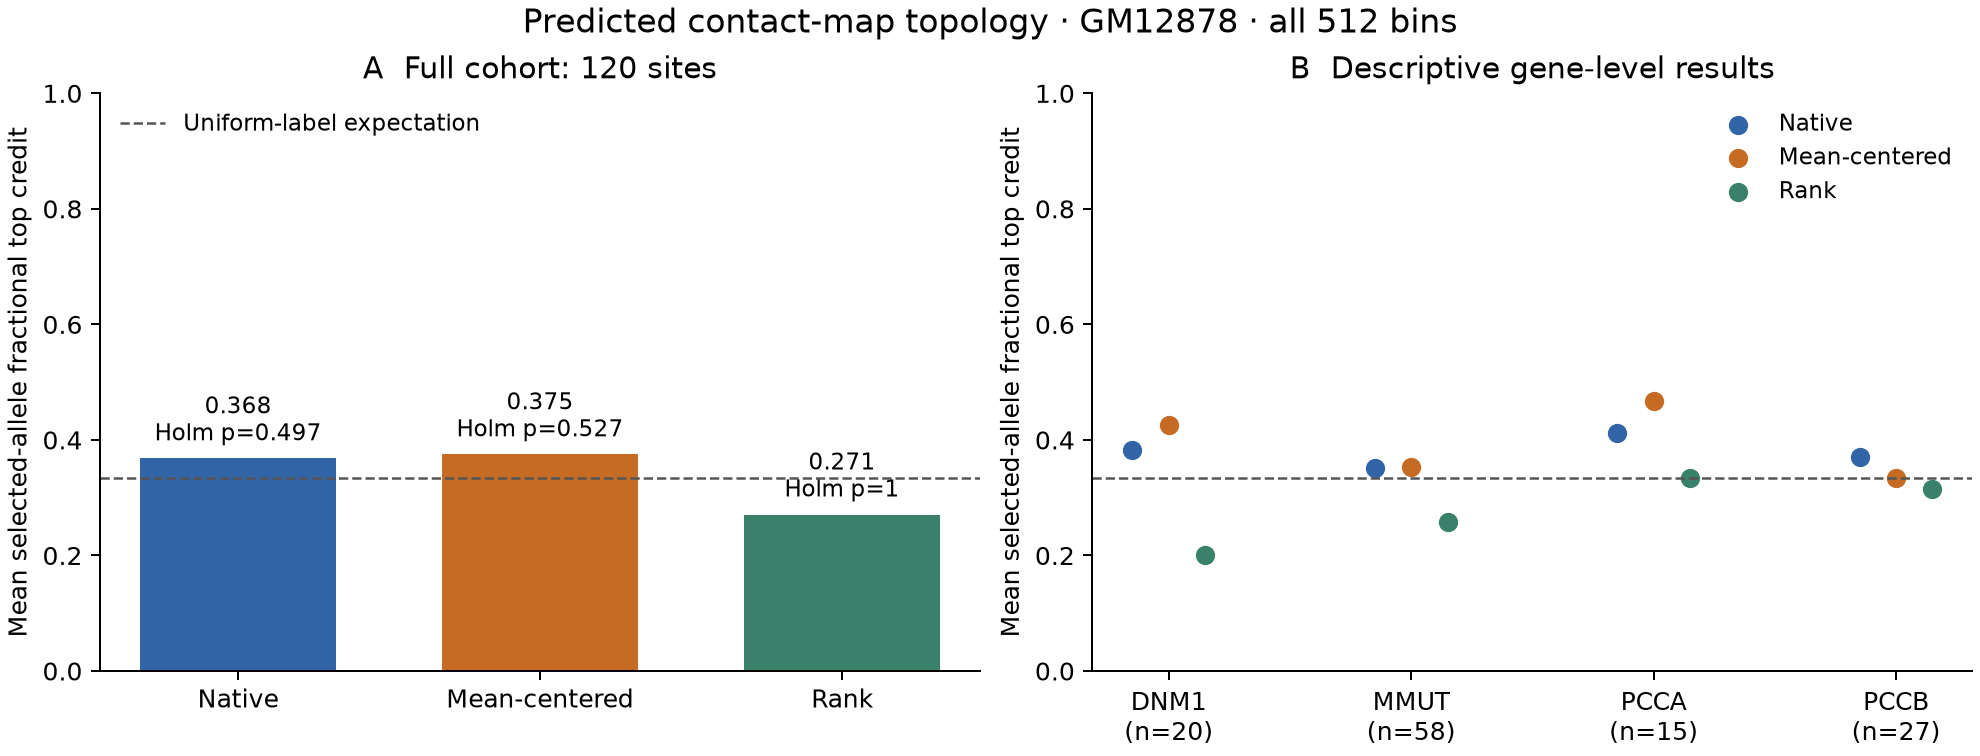
\includegraphics[keepaspectratio,alt={Discovery selected-credit estimates with consequence-aware controls}]{figures/figure_4_genomic_topology.png}}

\par\noindent\begin{minipage}{\linewidth}

\textbf{Figure 4. Discovery selected-credit estimates.} Fractional top
credit at all 120 discovery sites, with uniform-label expectation 1/3.
Gene points are descriptive. Holm values use the full four-test primary
family. No gene was selected by its result.

\end{minipage}\par

\subsubsection{Consequence controls from the retained within-site
audit}\label{consequence-controls-from-the-retained-within-site-audit}

The incorporated Atlas audit illustrates the complementary effect of
clinical ascertainment and consequence. In the seven-gene expansion,
ranking AVI Euclidean distance from a background centroid placed the
ClinVar allele first at 1,095/1,238 nonsense or start-loss positions
(88\%) and 94/246 missense positions (38\%). Across all 1,490 coding
positions, including six synonymous positions, the observed first-choice
fraction was 1,192/1,490 (0.800), below the exploratory model-free
consequence-severity rule's expected 0.817. This supports including
strong non-topological explanations before interpreting enrichment.

Ten of 66 coding comparisons remained significant under the
matched-consequence null, compared with 37 under the uniform null. Given
37 significant comparisons under the uniform null, the prespecified
``mainly consequence class'' criterion required nine or fewer under
consequence matching. The observed count of ten did not meet that
criterion. Eligible cohorts also differed (452 versus 1,490 AVI
positions), so this was not a fixed-cohort null comparison. Three
redraws reproduced 37/10, but simultaneous Monte Carlo count enclosures
of 36--37 and 8--11 could not certify the criterion (Additional file 3).

Missense AVI mean-statistic enrichment persisted under the
consequence/mutation null (reported q=0.00132), while the observed mean
selected-minus-largest-other margin remained negative (−0.0128 versus
null mean −0.0829). Outside chr13 it was −0.0407 versus −0.0785
(q=0.00165). The reported q-values are multiplicity-adjusted estimates
derived from raw p-values at the Monte Carlo simulation floor. The mean
selected-minus-largest-other margins remain negative despite enrichment
relative to the specified null. Three splicing scorers ranked the
selected allele first at 46, 47 and 47 of 63 other-intronic sites,
whereas no mean-statistic comparison was significant at 157
canonical-splice positions. Computational evidence may contribute to
clinical classifications {[}28,29{]}. Additional files 3 and 5 retain
these results, their Monte Carlo limitations, earlier contact-profile
results and all eligibility rules. Direct spatial REF--ALT comparisons
remove the external centroid but do not remove consequence,
ascertainment or label-circularity concerns.

\subsection{Discussion}\label{discussion}

The GM12878 discovery and new-locus replication reproduce the observed
centering-associated tie resolution. In those two cohorts, centering
operated on numerically saturated branches of the bottleneck translation
path. It resolved native ties while preserving every strict native
leader and every individual interval lifetime. The path audit makes this
behavior inspectable: a reader can identify the anchor, see which
comparisons move, and determine which allele decisions remain unresolved
at the stated tolerance.

The IMR-90 test separates general audit utility from the earlier
saturation pattern: the strengthened bounds added 42 decisions across
six genes even though three comparisons failed numerical saturation.
Both simple and strengthened bounds retained unresolved sets at all
three exceptional sites. This prospective check supports use of the
bounded audit beyond a dataset in which every endpoint happens to
saturate. It does not establish universal saturation or transfer to an
independent model.

The clinical and representational findings answer different questions.
The discovery analysis did not establish selected-allele enrichment
after its declared multiplicity corrections. GM12878 replication
produced more unique rankings but a descriptive decrease in
selected-allele credit; the paired IMR-90 change was positive. The
direction of this descriptive change therefore depended on the track,
and RMS baselines exceeded centered H1 in both tracks. The original
within-site results likewise required consequence and mutation controls.
A summary's ability to distinguish alternatives must be assessed against
the information it retains and the way the evaluated labels were
selected.

The audit combines established stability and matching results into a
procedure for identifying centered-ranking decisions from uncentered
inputs and describing the path after both endpoints are evaluated. Its
empirical contribution is the gain in decision coverage demonstrated
prospectively on a second AlphaGenome track, with unresolved cases
retained explicitly. The new-locus analysis, consequence controls and
simpler baselines place these decisions in their genomic and statistical
context.

The source maps are predictions from one model on GM12878 and IMR-90
tracks. The paired IMR-90 extension reuses the seven replication loci;
it increases track coverage without adding independent loci or model
architectures. The selected ClinVar sites were not curated for
experimentally verified chromatin-contact disruption. At each site, one
alternate is ClinVar-selected and the other two are unselected; these
alternatives do not form an independently validated
pathogenic-versus-benign set. The eleven loci and overlapping
within-gene windows limit generalization; the gene-balanced replication
also differs from the eligible panel's consequence distribution.
Historical scorer exposure and unestablished model-training independence
limit stronger holdout claims.

Delivered values lie on a bfloat16 grid. This observation, together with
the finite matching geometry, makes numerical resolution relevant to
ties. It does not establish that quantization causes every tie or
saturation event; a higher-precision comparison would be needed to
isolate that contribution. The recorded PH rounding bounds address added
filtration conversion. The practical solver allowances and numerical
witness checks do not constitute complete real-arithmetic certificates.
Exact theoretical path bounds remain conditional on valid endpoint
errors when used for rigorous numerical enclosures.

Mean centering removes a declared additive offset and retains relative
diagram-location information. Neither the mean alone nor the native
scalar distance determines the directional response. The alternative
shift-invariant distance optimizes over origins and addresses a
different target; it was not substituted for the frozen endpoint.
Abstract H1 diagrams also discard genomic labels. Observed-contact data,
perturbations with known local structural effects and
coordinate-sensitive comparisons would be required to connect the
present model-output audit to physical chromosome architecture. Those
are open validation tasks.

\subsection{Conclusions}\label{conclusions}

The audit uses information from uncentered maps to identify centered
allele-ranking leaders while retaining unresolved cases. In the
prospective IMR-90 test, strengthened bounds increased coverage from 7
of 84 to 49 of 84 sites, adding 42 decisions across six genes; 35 sites
remained unresolved. All predicted leaders agreed with separately
evaluated centered distances, although universal numerical saturation
did not transfer. These findings support the audit's use on the two
evaluated AlphaGenome tracks. They do not establish improved clinical
prediction. Validation with other model architectures and experimental
contact data remains future work.

\subsection{Abbreviations}\label{abbreviations}

AI: artificial intelligence; ALT: alternate allele; AVI: AlphaGenome
Variant Impact; BH: Benjamini--Hochberg; BY: Benjamini--Yekutieli; H1:
degree-one persistent homology; PH: persistent homology; P/LP:
pathogenic or likely pathogenic; REF: reference allele; RMS: root mean
square.

\subsection{Declarations}\label{declarations}

\subsubsection{Ethics approval and consent to
participate}\label{ethics-approval-and-consent-to-participate}

Not applicable. This computational study uses public variant annotations
and model predictions, with no new participant recruitment or
intervention.

\subsubsection{Consent for publication}\label{consent-for-publication}

Not applicable. No identifiable participant information is reported.

\subsubsection{Availability of data and
materials}\label{availability-of-data-and-materials}

The retained within-site analysis is archived in Zenodo {[}25{]}. Anchor
Audit Toolkit is available from its source repository {[}26{]}; the
complete study archive is preserved in the versioned v0.2.0 release
{[}27{]}. The full archive contains the stored maps, paired calls, full
diagrams, frozen protocols, computational source and execution records,
including the earlier reproduction capsule. Its three download parts
have checksums and reassembly instructions. Additional file 7 supplies a
compact scalar-verification archive for checking the paired-track
counts, bounds and credits without model access; these scalar results
alone cannot regenerate persistence diagrams. The release README
distinguishes full stored-map replay from scalar verification and
acquisition preparation.

Project: Anchor Audit Toolkit. Home page: reference {[}26{]}. Study code
and data archive: v0.2.0 {[}27{]}. Operating systems: platform
independent; Python reference CLI and JavaScript browser demo. The
reference toolkit requires Python 3.10 or later, with no runtime
dependencies; the optional accelerated stack requires Python 3.12 or
later and the pinned compatible packages. Original software license:
MIT. AlphaGenome outputs and substantial derivatives, including the
derived genomic numerical results and Figures 2--4, S4.1 and S6.1, are
subject to the legally binding AlphaGenome Output Terms {[}30{]},
separately from the software license. The archive includes those terms,
required notices and a modification record. Processing includes mean
centering, persistence analysis, ranking and visualization; saved raw
map arrays retain their original bytes. No blanket MIT or Creative
Commons license over provider outputs is asserted.

\subsubsection{Competing interests}\label{competing-interests}

The author declares no competing financial or nonfinancial interests.

\subsubsection{Funding}\label{funding}

This work received no specific grant or institutional funding.

\subsubsection{Authors' contributions}\label{authors-contributions}

P.I. developed the research program and is responsible for the study
design, analyses, interpretation and manuscript. Generative-AI
assistance is disclosed in Methods. Final author approval of this
proposed revision remains pending.

\subsubsection{Acknowledgements}\label{acknowledgements}

Not applicable.

\subsection{Additional files}\label{additional-files}

\textbf{Additional file 1 (PDF): Vertex thinning.} Finite-bin extinction
argument and map-specific refinement; a scope control, not an empirical
read-depth analysis.

\textbf{Additional file 2 (PDF): Anchor theory.} Proofs, matching
arguments, invariance comparisons and counterexamples supporting the
audit.

\textbf{Additional file 3 (PDF): Monte Carlo scope.} Simulation-floor
precision and interpretation of retained within-site tests.

\textbf{Additional file 4 (PDF): Track portability.} Frozen design,
gene-level outcomes, tolerances, baselines and exploratory exception
paths.

\textbf{Additional file 5 (PDF): Retained within-site audit.} Complete
incorporated methods and results, including adverse controls and
ascertainment limitations.

\textbf{Additional file 6 (PDF): Reproducibility details.} Acquisition,
replay, numerical checks, preservation records and the fixed-site
contact-map illustration.

\textbf{Additional file 7 (ZIP): Compact scalar-verification archive.}
Source, environment records, protocols and derived scalar data for
checking bounds, ranking sets and selected-allele credits. Recomputing
persistence diagrams requires the saved maps in the separate full study
archive.

\subsection{References}\label{references}

\begin{enumerate}
\def\labelenumi{\arabic{enumi}.}
\tightlist
\item
  Avsec Z, Latysheva N, Cheng J, et al.~Advancing regulatory variant
  effect prediction with AlphaGenome. \emph{Nature}.
  2026;649:1206--1218.
  \href{https://doi.org/10.1038/s41586-025-10014-0}{doi:10.1038/s41586-025-10014-0}.
\item
  Cheng J, Taylor KR, Nicolaisen L, et al.~AlphaGenome Atlas: in silico
  mutagenesis of the entire human genome improves prioritization and
  interpretation of non-coding variants. \emph{medRxiv}, preprint, 2026.
  \href{https://doi.org/10.64898/2026.09.16.26363192}{doi:10.64898/2026.09.16.26363192}.
\item
  Sauerwald N, Shen Y, Kingsford C. Topological Data Analysis Reveals
  Principles of Chromosome Structure in Cellular Differentiation.
  \emph{WABI 2019, LIPIcs}. 2019;143:23:1--23:16.
  \href{https://doi.org/10.4230/LIPIcs.WABI.2019.23}{doi:10.4230/LIPIcs.WABI.2019.23}.
\item
  Chiang Z, Wu Y. Persistent homology-based multiscale Hi-C analysis
  uncovers TADs-mediated gene regulation. \emph{Scientific Reports}.
  2026;16:22347.
  \href{https://doi.org/10.1038/s41598-026-52335-8}{doi:10.1038/s41598-026-52335-8}.
\item
  Mustafa A. HICTDA: A Persistent Homology Framework for Multiscale
  Identification of Topologically Associating Domains (TADS) in Hi-C
  Data. \emph{F1000Research}. 2026;15:1752, version 1, awaiting peer
  review.
  \href{https://doi.org/10.12688/f1000research.189367.1}{doi:10.12688/f1000research.189367.1}.
\item
  Giusti C, Pastalkova E, Curto C, Itskov V. Clique topology reveals
  intrinsic geometric structure in neural correlations. \emph{PNAS}.
  2015;112:13455--13460.
  \href{https://doi.org/10.1073/pnas.1506407112}{doi:10.1073/pnas.1506407112}.
\item
  Petri G, Expert P, Turkheimer F, et al.~Homological scaffolds of brain
  functional networks. \emph{Journal of the Royal Society Interface}.
  2014;11:20140873.
  \href{https://doi.org/10.1098/rsif.2014.0873}{doi:10.1098/rsif.2014.0873}.
\item
  Imakaev M, Fudenberg G, McCord RP, et al.~Iterative correction of Hi-C
  data reveals hallmarks of chromosome organization. \emph{Nature
  Methods}. 2012;9:999--1003.
  \href{https://doi.org/10.1038/nmeth.2148}{doi:10.1038/nmeth.2148}.
\item
  Sheehy D, Kisielius O, Cavanna N. Computing the Shift-Invariant
  Bottleneck Distance for Persistence Diagrams. \emph{Proceedings of the
  30th Canadian Conference on Computational Geometry}. 2018:78--84.
  \href{https://donsheehy.net/research/cavanna18computing.pdf}{Primary
  paper}.
\item
  Cao Y, Monod A, Vlontzos A, Schmidtke L, Kainz B. Topological
  information retrieval with dilation-invariant bottleneck comparative
  measures. \emph{Information and Inference}. 2023;12(3):1964--1996.
  \href{https://academic.oup.com/imaiai/article/12/3/1964/7217093}{Publisher
  article}.
\item
  May NH, Krishnamoorthy B, Gambill P. A Normalized Bottleneck Distance
  on Persistence Diagrams and Homology Preservation under Dimension
  Reduction. \emph{La Matematica}. 2024;3:1486--1509.
  \href{https://doi.org/10.1007/s44007-024-00130-0}{doi:10.1007/s44007-024-00130-0}.
\item
  Smaruj PN, Kelley DR, Fudenberg G. Sequence design for
  three-dimensional genome folding using Akita Semifreddo. \emph{Genome
  Biology}. Accepted article published 26 October 2026.
  \href{https://doi.org/10.1186/s13059-026-04313-6}{doi:10.1186/s13059-026-04313-6}.
\item
  Google DeepMind.
  \href{https://www.alphagenomedocs.com/exploring_model_metadata.html}{Model
  output metadata}. AlphaGenome documentation, accessed 28 October 2026.
\item
  Google DeepMind.
  \href{https://www.alphagenomedocs.com/api/generated/alphagenome.models.variant_scorers.ContactMapScorer.html}{ContactMapScorer}
  and \href{https://www.alphagenomedocs.com/variant_scoring.html}{How
  variant scoring works}. AlphaGenome documentation, accessed 28 October
  2026.
\item
  Chazal F, de Silva V, Glisse M, Oudot S. \emph{The Structure and
  Stability of Persistence Modules}. SpringerBriefs in Mathematics.
  2016.
  \href{https://doi.org/10.1007/978-3-319-42545-0}{doi:10.1007/978-3-319-42545-0}.
  Earlier version:
  \href{https://arxiv.org/abs/1207.3674v3}{arXiv:1207.3674v3}, 2013.
\item
  Hong H, Jiang S, Li H, et al.~DeepHiC: A generative adversarial
  network for enhancing Hi-C data resolution. \emph{PLOS Computational
  Biology}. 2020;16:e1007287.
  \href{https://doi.org/10.1371/journal.pcbi.1007287}{doi:10.1371/journal.pcbi.1007287}.
\item
  Landrum MJ, Chitipiralla S, Kaur K, et al.~ClinVar: updates to support
  classifications of both germline and somatic variants. \emph{Nucleic
  Acids Research}. 2025;53:D1313--D1321.
  \href{https://doi.org/10.1093/nar/gkae1090}{doi:10.1093/nar/gkae1090}.
\item
  Holm S. A Simple Sequentially Rejective Multiple Test Procedure.
  \emph{Scandinavian Journal of Statistics}. 1979;6(2):65--70.
  \href{https://www.jstor.org/stable/4615733}{Journal archive}.
\item
  Benjamini Y, Yekutieli D. The control of the false discovery rate in
  multiple testing under dependency. \emph{Annals of Statistics}.
  2001;29:1165--1188.
  \href{https://doi.org/10.1214/aos/1013699998}{doi:10.1214/aos/1013699998}.
\item
  Cheng J, Novati G, Pan J, et al.~Accurate proteome-wide missense
  variant effect prediction with AlphaMissense. \emph{Science}.
  2023;381:eadg7492.
  \href{https://doi.org/10.1126/science.adg7492}{doi:10.1126/science.adg7492}.
\item
  McLaren W, Gil L, Hunt SE, et al.~The Ensembl Variant Effect
  Predictor. \emph{Genome Biology}. 2016;17:122.
  \href{https://doi.org/10.1186/s13059-016-0974-4}{doi:10.1186/s13059-016-0974-4}.
\item
  Phipson B, Smyth GK. Permutation P-values should never be zero:
  calculating exact P-values when permutations are randomly drawn.
  \emph{Statistical Applications in Genetics and Molecular Biology}.
  2010;9:Article 39.
  \href{https://doi.org/10.2202/1544-6115.1585}{doi:10.2202/1544-6115.1585}.
\item
  Benjamini Y, Hochberg Y. Controlling the false discovery rate: a
  practical and powerful approach to multiple testing. \emph{Journal of
  the Royal Statistical Society, Series B}. 1995;57:289--300.
  \href{https://doi.org/10.1111/j.2517-6161.1995.tb02031.x}{doi:10.1111/j.2517-6161.1995.tb02031.x}.
\item
  Iben P. Pre-specified analysis plan: expanded-panel replication of a
  within-site audit of AlphaGenome Atlas predictions. Zenodo, version
  1.0, 2026.
  \href{https://doi.org/10.5281/zenodo.23524782}{doi:10.5281/zenodo.23524782}.
\item
  Iben P. Reproducibility package for ``What do within-site comparisons
  of AlphaGenome Atlas predictions measure? An audit at ClinVar sites in
  11 genes''. Zenodo, version 1.0, 2026.
  \href{https://doi.org/10.5281/zenodo.23537469}{doi:10.5281/zenodo.23537469}.
\item
  Iben P. Anchor Audit Toolkit. Source repository.
  \url{https://github.com/patrickiben/contact-map-anchor-audit}.
  Accessed 28 October 2026.
\item
  Iben P. Anchor Audit Toolkit and full study reproducibility archive
  v0.2.0.
  \url{https://github.com/patrickiben/contact-map-anchor-audit/releases/tag/v0.2.0}.
  Accessed 28 October 2026.
\item
  Richards S, Aziz N, Bale S, et al.~Standards and guidelines for the
  interpretation of sequence variants: a joint consensus recommendation
  of the American College of Medical Genetics and Genomics and the
  Association for Molecular Pathology. \emph{Genetics in Medicine}.
  2015;17:405--424.
  \href{https://doi.org/10.1038/gim.2015.30}{doi:10.1038/gim.2015.30}.
\item
  Pejaver V, Byrne AB, Feng BJ, et al.~Calibration of computational
  tools for missense variant pathogenicity classification and ClinGen
  recommendations for PP3/BP4 criteria. \emph{American Journal of Human
  Genetics}. 2022;109:2163--2177.
  \href{https://doi.org/10.1016/j.ajhg.2022.10.013}{doi:10.1016/j.ajhg.2022.10.013}.
\item
  Google DeepMind. AlphaGenome Output Terms of Use. Effective 9 October
  2026.
  \url{https://storage.googleapis.com/alphagenome/terms/20260909/AlphaGenome-Output-Terms-of-Use.pdf}.
  Accessed 28 October 2026.
\end{enumerate}

\end{document}
